\documentclass[a4paper,12pt]{article}
\usepackage[utf8]{inputenc}
\usepackage{geometry}
\usepackage{fancyhdr}
\usepackage{listings}
\usepackage{xcolor}
\usepackage{graphicx}
\usepackage{float}

% Margins
\geometry{left=15mm, right=15mm, top=25mm, bottom=15mm}

% Header/Footer
\pagestyle{fancy}
\fancyhf{}
\renewcommand{\headrulewidth}{0pt}
\rfoot{Page \thepage}

\fancypagestyle{firstpage}{
    \fancyhf{}
    \lhead{
        \small \textbf{Name:} Mrigaj Shaw \\ 
        \small \textbf{Roll No:} 2024CSB041
    }
    \chead{\LARGE \textbf{Assignment 4}} 
    \rfoot{Page \thepage}
    \renewcommand{\headrulewidth}{1pt}
}

% Code Style
\definecolor{codegreen}{rgb}{0,0.6,0}
\definecolor{codegray}{rgb}{0.5,0.5,0.5}
\definecolor{codepurple}{rgb}{0.58,0,0.82}
\definecolor{backcolour}{rgb}{0.95,0.95,0.92}

\lstdefinestyle{MyCodeStyle}{
    backgroundcolor=\color{backcolour},   
    commentstyle=\color{codegreen},
    keywordstyle=\color{magenta},
    numberstyle=\tiny\color{codegray},
    stringstyle=\color{codepurple},
    basicstyle=\ttfamily\footnotesize,
    breakatwhitespace=false,         
    breaklines=true,                 
    keepspaces=true,                 
    numbers=left,                    
    numbersep=5pt,                  
    showspaces=false,                
    showstringspaces=false,
    showtabs=false,                  
    tabsize=4
}
\lstset{style=MyCodeStyle}

\begin{document}
\thispagestyle{firstpage}

% --- Problem1 ---
\section*{Problem 1: Fibonacci Series}
\textbf{Problem Statement:}\\
In a smart agriculture system, many sensors are placed in fields to collect data such as soil moisture, temperature, and humidity. These sensors send the collected data to a central server through a wireless network. Sometimes, due to weak network connectivity, data packets fail to reach the server successfully. To handle this situation, the system waits for some time before trying to send the data again. Instead of waiting for the same time every time, the system increases the waiting time gradually to reduce network congestion. One simple method used in many computer networks is the Fibonacci backoff strategy, where the waiting time follows the Fibonacci sequence. For example, if the first retry fails, the system waits 1 second, then 1 second, then 2 seconds, then 3 seconds, then 5 seconds, 8 seconds, and so on. However, when the number of retries becomes large, calculating Fibonacci numbers using the simple recursive method becomes slow because the same values are calculated many times. Therefore, developers want to compare different methods to calculate Fibonacci numbers efficiently.

Write a C program to compute the $n$-th Fibonacci number using the following two approaches:
\begin{enumerate}
    \item \textbf{Recursive Method:} Implement the traditional recursive Fibonacci algorithm where each value is calculated using repeated function calls.
    \item \textbf{Dynamic Programming Method:} Implement the Fibonacci algorithm using Dynamic Programming (Memoization or Tabulation) where previously calculated values are stored and reused.
\end{enumerate}

After implementing both methods, perform a comparative analysis based on the following:
\begin{itemize}
    \item Time Complexity in the best case, average case, and worst case.
    \item Space Complexity in the best case, average case, and worst case.
    \item Execution performance when calculating large Fibonacci numbers.
\end{itemize}

\newpage
\subsection*{Code}
\lstinputlisting[language=C]{Problem1/FibonacciDP.c}

\newpage
\subsection*{Output}
\begin{figure}[H]
    \centering
    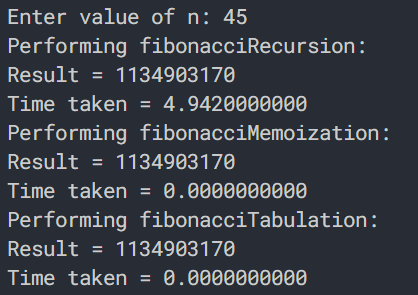
\includegraphics[width=0.9\textwidth]{Problem1/Problem 1.png}
\end{figure}

\newpage
\subsection*{Inference}
\begin{itemize}
    \item \textbf{Recursive Approach:} The naive recursive method exhibits an exponential time complexity of $O(2^n)$ (more precisely, bounded by the golden ratio) because it repeatedly solves the same overlapping subproblems. The space complexity is $O(n)$ due to the maximum depth of the function call stack. For larger values of $n$ (e.g., $n > 40$), the execution time becomes exceptionally slow and impractical.
    \item \textbf{Dynamic Programming Approach:} The DP method (memoization or tabulation) reduces the time complexity drastically to a linear $O(n)$ by storing previously computed values in an array. The space complexity is $O(n)$ to store the array, though a tabulation approach can be further optimized to $O(1)$ space by only tracking the last two variables.
    \item \textbf{System Application:} In the context of the smart agriculture system's network congestion, calculating the Fibonacci backoff must be instantaneous to quickly evaluate network retries. The DP approach ensures that the server does not waste CPU cycles computing wait times, making it the clear optimal choice as the number of retries scales.
\end{itemize}

\newpage

% --- Problem2 ---
\section*{Problem 2: Matrix Chain Multiplication}
\textbf{Problem Statement:}\\
In many cloud computing and machine learning systems, large numbers of matrices are multiplied together to perform computations such as data transformations, neural network training, and image processing. Suppose several matrices need to be multiplied in sequence:
$$A_{1}, A_{2}, A_{3}, \dots, A_{n}$$

Even though the final multiplication result remains the same, the number of calculations required can be very different depending on the order in which the matrices are multiplied. For example, suppose we have three matrices with dimensions:
\begin{itemize}
    \item ($10 \times 30$)
    \item ($30 \times 5$)
    \item ($5 \times 60$)
\end{itemize}

If we change the order of multiplication, the total number of scalar multiplications required will also change. Some orders require fewer calculations and therefore execute faster. To improve performance, the system must determine the best order of multiplying matrices that minimizes the total number of scalar multiplications.

Write a C program to determine the minimum number of scalar multiplications required to multiply a sequence of matrices using the following approaches:
\begin{enumerate}
    \item \textbf{Recursive Approach:} Implement a recursive algorithm that checks all possible ways of multiplying the matrices and finds the minimum cost.
    \item \textbf{Dynamic Programming Approach (Matrix Chain Multiplication):} Implement the dynamic programming solution that stores intermediate results in a table and avoids repeated calculations.
\end{enumerate}

After implementing both methods, perform a comparative analysis based on the following factors:
\begin{itemize}
    \item Time Complexity in the best case, average case, and worst case.
    \item Space Complexity in the best case, average case, and worst case.
    \item Performance when the number of matrices increases.
\end{itemize}

\newpage
\subsection*{Code}
\lstinputlisting[language=C]{Problem2/MatrixChainMultiplication.c}

\newpage
\subsection*{Output}
\begin{figure}[H]
    \centering
    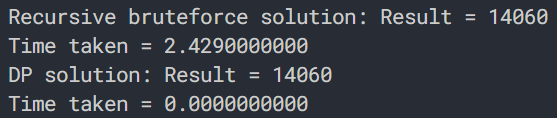
\includegraphics[width=0.9\textwidth]{Problem2/Problem 2.png}
\end{figure}

\newpage
\subsection*{Inference}
The analysis of the Matrix Chain Multiplication problem yields the following observations regarding computational optimization:
\begin{itemize}
    \item \textbf{Recursive Approach:} The brute-force recursive method evaluates all possible parenthesizations to find the minimum cost. This leads to an exponential time complexity of $\Omega(2^n)$ (specifically proportional to the Catalan numbers). The space complexity is $O(n)$ for the recursion stack. This approach is highly inefficient for any sequence longer than a few matrices.
    \item \textbf{Dynamic Programming Approach:} By utilizing a bottom-up DP table, the time complexity is reduced to $O(n^3)$, where $n$ is the number of matrices. The space complexity increases to $O(n^2)$ to maintain the minimum scalar multiplication cost table and the split marker ($k$) tracking table. There is wasted space too as an upper triangle matrix is used for the DP table.
    \item \textbf{Performance Impact:} For cloud computing systems handling massive data transformations or neural networks, multiplying matrices in a sub-optimal order can cause millions of unnecessary scalar computations. The $O(n^3)$ computational overhead to determine the optimal split is negligible compared to the time saved during the actual heavy matrix multiplications.
\end{itemize}.

\newpage

% --- Problem3 ---
\section*{Problem 3: $0/1$ Knapsack Problem}
\textbf{Problem Statement:}\\
A delivery and logistics company transports packages using trucks that have a maximum weight capacity. The company must decide which packages should be loaded into a truck so that the total profit from delivered packages is as high as possible, without exceeding the weight limit of the truck. Each package has two properties:
\begin{itemize}
    \item \textbf{Weight:} how much space or load it occupies in the truck
    \item \textbf{Profit (Value):} the benefit gained from delivering that package
\end{itemize}

Since each package can either be selected or not selected, this problem is known as the $0/1$ Knapsack Problem. When the number of packages becomes large, checking all possible combinations of packages becomes very slow. Therefore, more efficient algorithms are needed.

Write a C program to solve the $0/1$ Knapsack Problem using the following approaches:
\begin{enumerate}
    \item \textbf{Recursive / Brute Force Approach:} Implement a recursive solution that checks all possible combinations of packages to find the maximum profit.
    \item \textbf{Dynamic Programming Approach:} Implement the dynamic programming solution using a table where intermediate results are stored to avoid repeated calculations.
\end{enumerate}

After implementing both methods, perform a comparative analysis based on:
\begin{itemize}
    \item Time Complexity in the best case, average case, and worst case.
    \item Space Complexity in the best case, average case, and worst case.
    \item Efficiency when the number of packages becomes very large.
\end{itemize}

\newpage
\subsection*{Code}
\lstinputlisting[language=C]{Problem3/KnapSack01.c}

\newpage
\subsection*{Output}
\begin{figure}[H]
    \centering
    
\includegraphics[width=0.9\textwidth]{Problem3/Problem3.png}
\end{figure}

\newpage
\subsection*{Inference}
The comparative analysis for the $0/1$ Knapsack problem highlights the necessity of algorithmic optimization in logistics and resource allocation:
\begin{itemize}
    \item \textbf{Recursive Approach:} The brute force strategy acts as a decision tree, exploring every possible subset of packages (either selecting or leaving each item). This results in an exponential time complexity of $O(2^n)$. The space complexity remains $O(n)$ strictly for the depth of the recursive call stack. This method causes the system to stall entirely as the package count increases.
    \item \textbf{Dynamic Programming Approach:} The DP tabulation method solves this overlapping subproblem structure in pseudo-polynomial time, specifically $O(n \cdot W)$, where $n$ is the number of packages and $W$ is the maximum weight capacity of the truck. The space complexity is $O(n \cdot W)$, though it can be theoretically optimized to $O(W)$ by only keeping the current and previous rows of the DP table in memory.
    \item \textbf{Practical Efficiency:} For a delivery company, maximizing profit while strictly adhering to weight limits is a daily operational requirement. The DP approach provides an optimal, highly scalable solution for typical truck loads. However, it should be noted that if the weight capacity $W$ becomes astronomically large, the $O(n \cdot W)$ complexity could eventually introduce heavy memory consumption.
\end{itemize}

\newpage

\end{document}